\section{OLD}
\subsection{Escenas}
Desde un punto de vista formal, este juego, al igual que el resto de juegos, es una \textbf{aplicación gráfica interactiva} con renderizado en tiempo real \cite{libro_esi}. Este tipo de aplicaciones están construidas sobre un bucle de ejecución (llamado comúnmente \textbf{bucle de juego} en el ámbito del videojuego) el cual esta formado por tres pasos:
\begin{enumerate}
\item \textbf{Renderizar} una imagen a traves de la pantalla del usuario.
\item \textbf{Leer} la entrada que el usuario suministre.
\item \textbf{Modificar} el estado del programa, del cual depende la siguiente renderización.
\end{enumerate}
Cuando se trata de un videojuego, este sistema de renderizado es acompañado de sistemas de audio, simuladores de físicas y otros subsistemas que permita dotar al jugo de realismo e inmersividad.

En la gran mayoría de los videojuegos se pueden distinguir una serie de ``etapas'' o ``estados'', en cada uno de los cuales se ejecuta una lógica distinta independiente. En nuestro caso, cada una de las ``pantallas'' descritas en el apartado anterior serían uno de estos estados. La mayor parte de los motores de juego permiten e incluso fomentan que programador realice estas divisiones del juego ofreciendo implementaciones de estos estados. dependiendo del motor, estas divisiones se pueden llamar \textbf{salas, mundos o escenas}.

En Unity, los estados del juego reciben el nombre de \textbf{Escena} \footnote{https://docs.unity3d.com/Manual/CreatingScenes.html}. A grandes rasgos, las escenas son un conjunto de entidades de juego situadas en un entorno tridimensional. Estas entidades se encuentran organizadas en un \textbf{grafos de escena}, un tipo de estructura de datos que permite representar las relaciones jerárquicas que existen entre los distintos objetos del juego o ``nodos'' haciendo uso de un grafo dirigido sin hijos \cite{libro_esi}. El uso de este tipo de estructura permite gestionar con facilidad escenas tridimensionales complejas, permitiendo que se apliquen las operaciones transformaciones (como la traslación, rotación y escalado) de un nodo padre a todos sus nodos hijos de forma automática y facilita tareas como las búsquedas de entidades concretas.

\begin{figure}[h]
    \centering
    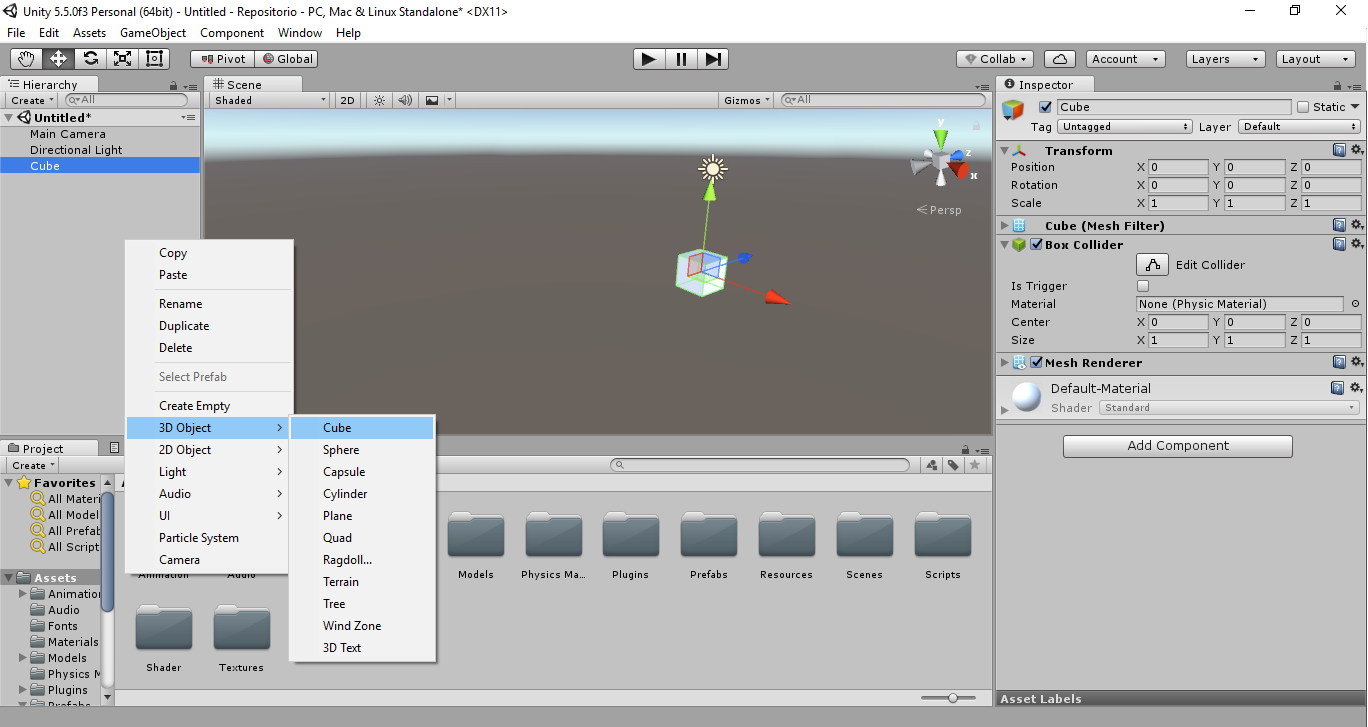
\includegraphics[width=0.8\textwidth]{images/estructura/old/escenas/editor}
    \caption{Editor de escenas de Unity.}
    \label{scene_editor}
\end{figure}

La suite de desarrollo de Unity incluye un editor de escenas, que permite la creación de estas mediante una interfaz gráfica. Las escenas se almacenan en archivos, de la misma forma que lo hacen las texturas o los modelos 3D, lo que facilita su gestión. Para la manipulación de escenas en tiempo de ejecución se utiliza el módulo \textbf{SceneManager} \footnote{https://docs.unity3d.com/ScriptReference/SceneManagement.SceneManager.html} que permite realizar cambios de escenas, cargar escenas en segundo plano y solapar varias escenas simultáneamente entre otras funciones. 

Para Virus Breaker, se optó por una estructura en cuatro Escenas: tres escenas de ``menú'' (menú de inicio, fin del juego y victoria) y una escena de juego, como puede verse en la figura \ref{scenes}. A continuación, se realizará una descripción de estos tipos de escenas

\begin{figure}[h]
	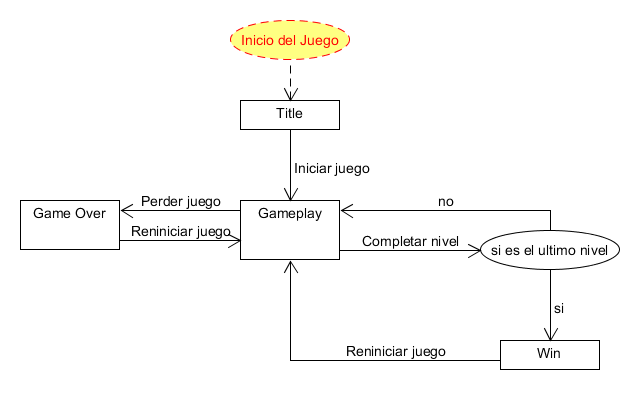
\includegraphics[width=0.8\textwidth]{images/estructura/old/escenas/scenes}
	\centering
	\caption{Diagrama de las escenas del juego}
	\label{scenes}
\end{figure}

\subsection{Escena de Juego}
La escena de juego es en la que ocurre \textbf{la acción del juego}, donde el jugador controla el personaje principal intentando completar los distintos niveles del juego. Como puede verse en el diagrama \ref{scenes}, se trata de la escena central del juego, a donde se dirigen el resto de las escenas. 

Se trata por tanto de \textbf{la escena más compleja del juego}, la que tiene mayor número de elementos e interacciones y en la que más tiempo pasa el jugador durante su partida. En la figura \ref{juego_detalles} se pueden ver detallados los distintos elementos de alto nivel que tiene esta escena:

\begin{figure}[h]
	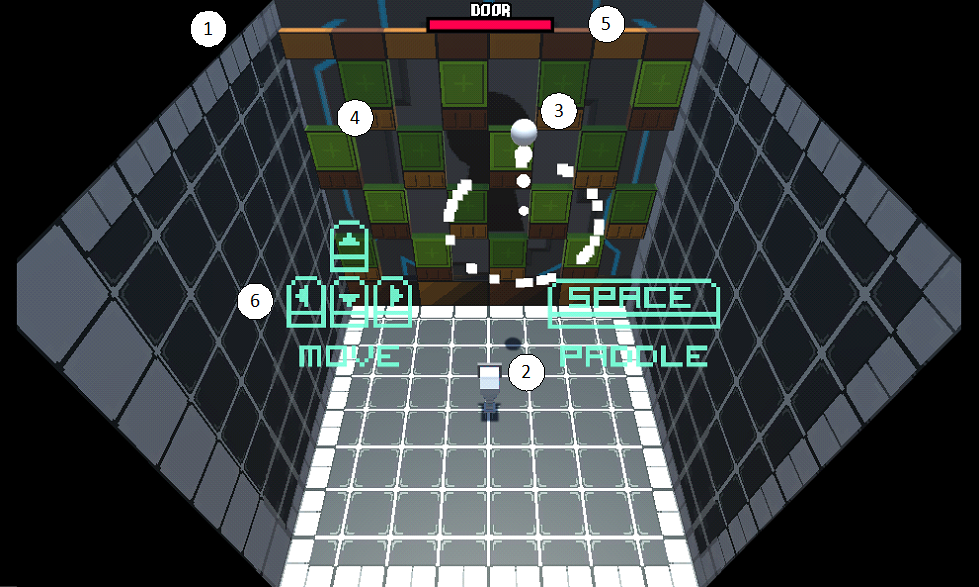
\includegraphics[width=0.8\textwidth]{images/estructura/old/escenas/juego_detalles}
	\centering
	\caption{Diagrama de las escenas del juego}
	\label{juego_detalles}
\end{figure}

\begin{enumerate}
\item\textbf{Sala}: La sala es el entorno en el que ocurre la partida. Está compuesta de tres paredes, suelo, techo y una puerta. La sala lleva el control del comportamiento general de la partida, encargándose de tareas como realizar transiciones de salas o activar y desactivar otros elementos según sea necesario.
\item\textbf{Personaje Principal}: Es el elemento sobre el que el jugador tiene un control directo. Puede moverse y crear una paleta. Su comportamiento se basa en una máquina de estados finitos.
\item\textbf{Pelota}: La pelota es un objeto que se mueve por la sala rebotando en sus paredes. Es posible el elemento más importante de la sala, ya que la mayor parta de interacciones entre objetos se realizan a través de la pelota
\item\textbf{Ladrillos}: Los ladrillos son unos elementos destructibles los cuales forman un muro que protege la puerta. Hay distintos tipos de ladrillos, cada uno con un comportamiento distinto.
\item\textbf{Resistencia de la puerta}: Se trata de una imagen que representa cuantos golpes necesita la puerta para abrirse.
\item\textbf{Tutorial en pantalla}: Son dos imágenes que muestran los controles del juego. Solo aparecen la primera vez que se inicia una partida, para no sobrecargar al jugador con información.
\end{enumerate}

\subsection{Objetos}
El comportamiento de un videojuego desarrollado en Unity viene dado por los \textbf{objetos} que hay en el juego y las interacciones que existen entre estos. Estos objetos deben de poder influir en distintos dominios del código, como el rende rizado, el sonido o las físicas, lo cual puede causar un importante problema de acoplamiento entre clases. Para solucionar este problema, Unity hace uso del patrón de diseño \textbf{Component}. Este patrón de diseño  
consiste en aislar los distintos dominios en clases \textbf{componentes}, las cuales pueden ser asociadas a un objeto contenedor de componentes \cite{game_programming_patterns}.

La clase contenedor de componentes en Unity se llama \textbf{GameObjects}\footnote{https://docs.unity3d.com/ScriptReference/GameObject.html}. Los GameObjets se instancian mediante el editor de Unity o mediante código con el método estático \textbf{Instantiate}\footnote{https://docs.unity3d.com/ScriptReference/Object.Instantiate.html}. Estos objetos carecen de funcionalidad, a excepción de una serie de métodos para realizar busquedas entre los GameObjets de una escena. La funcionalidad de los GameObjects viene dada por los objetos de la clase \textbf{Component}\footnote{https://docs.unity3d.com/Manual/Components.html}. Esta clase es padre de multitud de componentes con diferente funcionalidad. Algunos de los componentes más importantes de Unity son los siguientes:
\begin{itemize}
\item \textbf{Transform}\footnote{https://docs.unity3d.com/ScriptReference/Transform.html}: Este componente almacena la posición, rotación y escala del objeto en la escena. Cada transform tiene un padre, lo que permite aplicar las transformaciones de forma jerárquica. Como su función es tan importante, todos los GameObjets tienen uno asociado.
\item \textbf{Collider}\footnote{https://docs.unity3d.com/ScriptReference/Collider.html}: Los colliders son una familia de componentes que permiten realizar la detección de colisiones. Existen muchos tipos de colliders dependiendo de su forma (BoxCollider, SphereCollider...). La clase Collider y sus hijos interaccionan con el motor de físicas 3D de Unity, para las colisiones entre objetos en 2D se utiliza la familia de clases \textbf{Collider2D}.
\item \textbf{Rigidbody}\footnote{https://docs.unity3d.com/ScriptReference/Rigidbody.html}: Esta clase se utiliza para la simulación física de cuerpos rígidos en 3D. Rigidbody contiene metodos para aplicar cambios de posición y rotación a objetos basándose en su velocidad, aceleración, fricción... Para objetos en 2D, existe una clase equivalente llamada \textbf{Rigidbody2D}.
\item \textbf{Renderer}\footnote{https://docs.unity3d.com/ScriptReference/Renderer.html}: Este componente permite renderizar modelos y texturas en la escena. 
\item \textbf{Audio Source}\footnote{https://docs.unity3d.com/ScriptReference/AudioSource.html}: Los audio source son componentes que permiten a los objetos emitir clips sonido. El componente permite aplicar transformaciones en tiempo real a los sonidos que emite, como modificar su volumen o la altura de su tono.
\item \textbf{Animator}\footnote{https://docs.unity3d.com/ScriptReference/Animator.html}: Este componente permite añadir animaciones a los objetos. Se trata de una máquina de estados finitos que reproduce clips de animación de forma condicional. Estos clips pueden producir variaciones en las propiedades de otros componentes del objeto en función del tiempo.
\item \textbf{Particle System}\footnote{https://docs.unity3d.com/ScriptReference/ParticleSystem.html}: Es un componente que emite \textbf{partículas}, pequeñas imágenes 2D que permiten crear efectos visuales como fuego o explosiones.
\end{itemize}

Aparte de los componentes incluidos en Unity, los desarrolladores pueden construir sus propios componentes y añadirlos a los GameObjets. La clase \textbf{MonoBehaviour}\footnote{https://docs.unity3d.com/ScriptReference/MonoBehaviour.html
} se utiliza como base para estos componentes, incluye una serie de métodos llamados \textbf{eventos} que son llamados automáticamente cuando se cumplen ciertas condiciones, como por ejemplo al principio de la ejecución (evento Start).

En los siguientes apartados contienen una descripción de los distintos objetos que forman el juego. Estas descripciones describen la función del objeto, jerarquía de GameObjects que lo forman, los Componentes que tienen asociados y el código de los scripts que definen su comportamiento.


